\documentclass[ucs,10pt]{beamer}
\mode<presentation>
\hypersetup{pdfpagemode=FullScreen}

\usepackage{beamerthemesplit}
\usepackage{beamer_visser_um}


\usepackage{tikz}   
\usepackage{subfigure}
\usepackage{multimedia}
\usepackage{tcolorbox}
\usepackage{array,tabularx}
\usepackage{colortbl}

\setlength{\unitlength}{\textwidth}  % measure in textwidths 

\setbeamertemplate{sidebar right}{}
\setbeamertemplate{footline}{%
\hfill\usebeamertemplate***{navigation symbols}
\hspace{1cm}\insertframenumber{}/\inserttotalframenumber}


\title{Activity Monitoring and Prediction for Humans and NAO Humanoid Robots using 
	Wearable Sensors}
\author{Saminda Abeyruwan, \underline{Faisal Sikder}, Ubbo Visser, and Dilip Sarkar}
\institute{Department of Computer Science\\ University of Miami \\ \vspace{.25cm}}
\date{May 19, 2015}
\titlegraphic{\putat{-0.52}{-0.15}{
\includegraphics[height=1.5cm]{logos/theUlogo}}}


\begin{document}

%%%%%%%%%%%%%%%%%%%%%%%%%%%%%%%%%%%%%%%%%%%%%%%%%%%%%%%%%%%%%


\frame{\titlepage}

%\section*{Outline}
%\frame{
%  \frametitle{Outline}    
%  \tableofcontents
%}


%%%%%%%%%%%%%%%%%%%%%%%%%%%%%%%%%%%%%%%%%%%%%%%%%%%%%%%%%%%%%

\section{Introduction}
\subsection{Introduction}

\frame{
  \frametitle{Introduction}
  \setbeamercovered{transparent} 
  
  \begin{tcolorbox}[colback=green!5,colframe=darkgreen!90!black,title=Challenges]
  \begin{itemize}
	\item Activities (jogging, running) may cause a fall.
	
	\item  Damage to the human body or to the structural components of the robot.
	    		
	\item Immediate identification.
	
	\item Inexpensive wearable sensors.
  \end{itemize}
  \end{tcolorbox}  
  
}

%%%%%%%%%%%%%%%%%%%%%%%%%%%%%%%%%%%%%%%%%%%%%%%%%%%%%%%%%%%%%
\subsection{Motivation}
\subsubsection*{Motivation}
\frame{
	\frametitle{Motivation}
	\setbeamercovered{transparent}
	\begin{tcolorbox}[colback=green!5,colframe=darkgreen!90!black,title=Motivation]
	\begin{itemize}
	\item Humans and biped humanoid robots have almost identical motions.
	\item  Susceptible to 
	similar accidents.
	\item Same set of learning algorithms
			 	are suitable for both groups.
 	\item Off-the-shelf hardware components to develop our sensing tools.
 	\item Generalized approach for learning and predicting
 	activities of both groups.
 	
 	\item  Detection of falls for both humans and robots within a unified framework;
 	
	\end{itemize}
	\end{tcolorbox}
	
}

%%%%%%%%%%%%%%%%%%%%%%%%%%%%%%%%%%%%%%%%%%%%%%%%%%%%%%%%%%%%%

\section{Our Approach and Contributions}
\subsection{Devices}
\subsection{Framework}

\frame{
	\frametitle{Our Approach and Contributions}
	\setbeamercovered{transparent}
	
	\begin{tcolorbox}[colback=green!5,colframe=darkgreen!90!black,title=Devices]
	\begin{itemize}
				\item Configuration: 
				\begin{enumerate}
				\item Tiva C Series TM4C123G microcontroller board.
				\item Sensor Hub BoosterPack for sensing 9-axis motion.
				\item CC2533 BoosterPack for wireless networking.
				\end{enumerate}
				\item Software tools:				
				\begin{enumerate}
					 \item Setup the WSN, 
					 \item Collect data using WSN network, 
					 \item To learn from sample examples, and 
					 \item To monitor and predict events. 
				\end{enumerate} 
			\end{itemize}
	\end{tcolorbox}
	 
	
}


%%%%%%%%%%%%%%%%%%%%%%%%%%%%%%%%%%%%%%%%%%%%%%%%%%%%%%%%%%%%%


\frame{
	\frametitle{Our Approach and Contributions}
	\setbeamercovered{transparent} 
	\begin{tcolorbox}[colback=green!5,colframe=darkgreen!90!black,title=Framework]
		\begin{itemize}
				\item Generic functionalities to develop applications or 
				rational agents on embedded devices.
				\item Tools to develop modules and representations that execute on the 
				 microcontrollers. 
				\item ``$\mu$Energia'': \url{http://muenergia.saminda.org}
			\end{itemize}
	\end{tcolorbox}
	
}



%%%%%%%%%%%%%%%%%%%%%%%%%%%%%%%%%%%%%%%%%%%%%%%%%%%%%%%%%%%%%

\frame{
	\frametitle{Framework}
	\setbeamercovered{transparent} 
\begin{figure}[!ht]
\centering
\minipage{0.48\textwidth}
\begin{tcolorbox}[colback=white!5,colframe=darkgreen!90!black]
  \centering \includegraphics[width=0.5\linewidth]{figures/human_figure}
  %\caption{5 Vs 5}\label{fig:timePlot}
  \end{tcolorbox}
\endminipage \hspace{2mm}
\minipage{0.48\textwidth}
\begin{tcolorbox}[colback=white!5,colframe=darkgreen!90!black]
  \centering 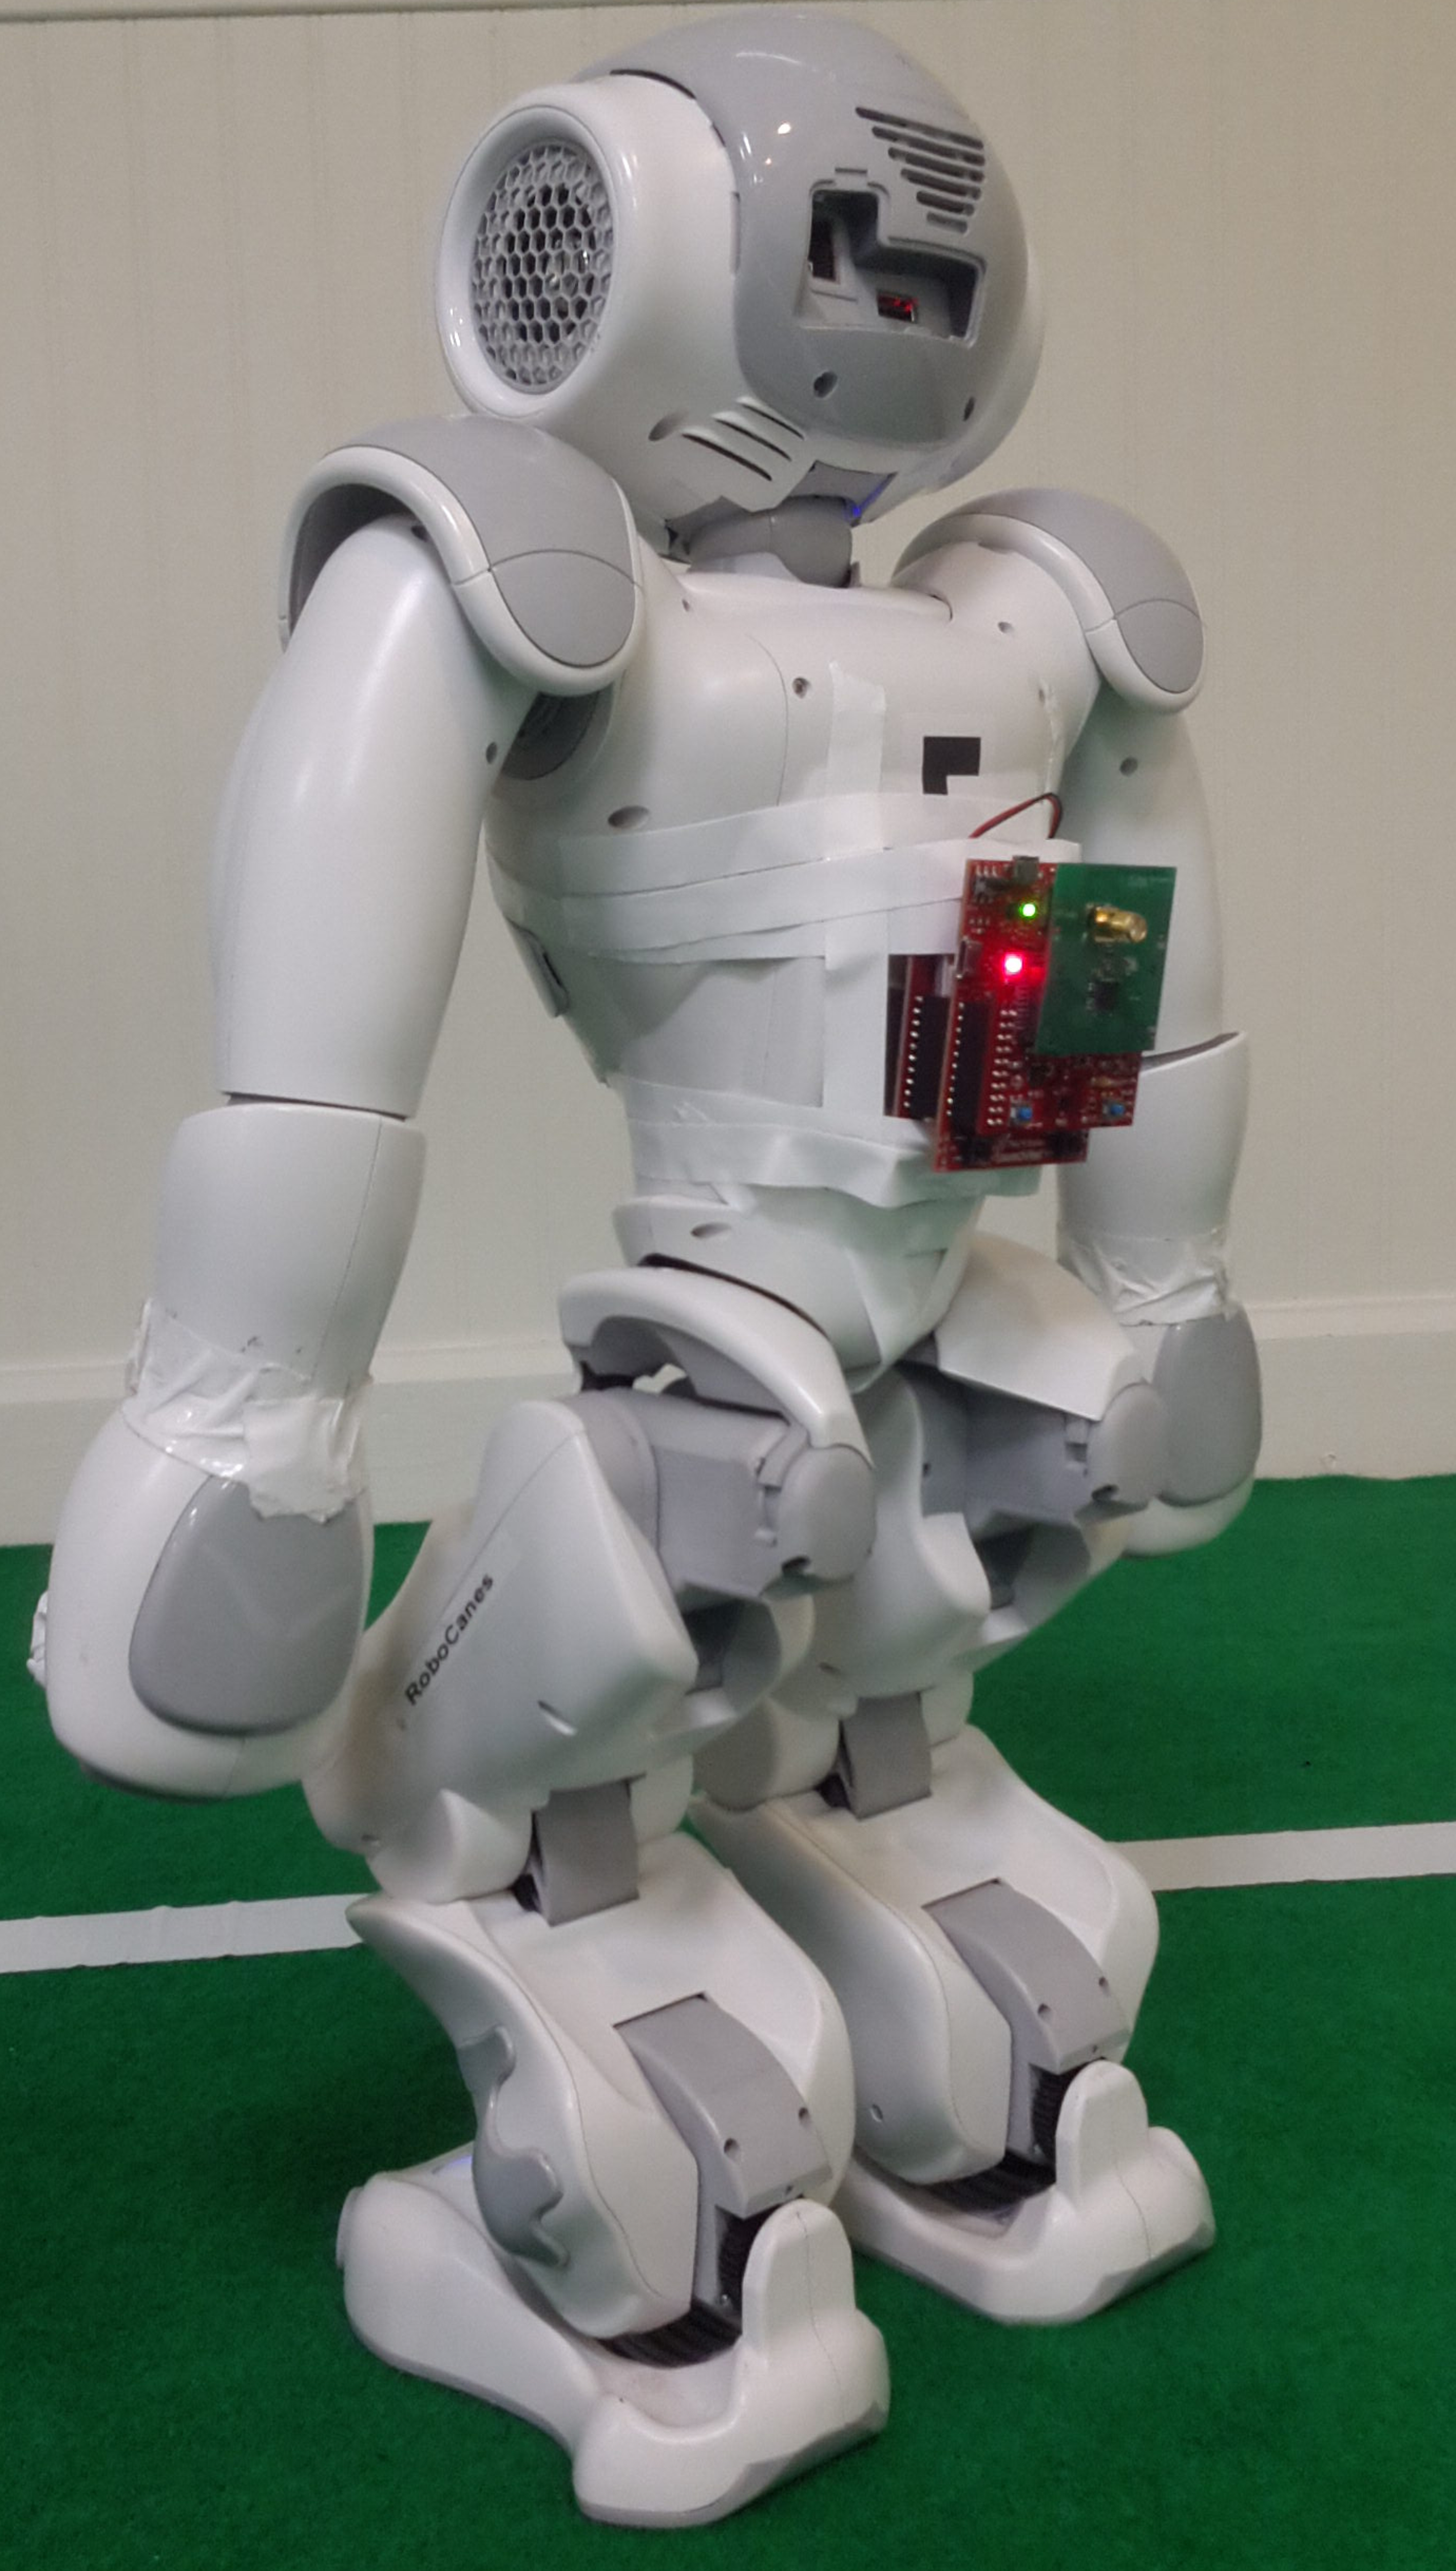
\includegraphics[width=0.45\linewidth]{figures/robot_figure}
  %\caption{7 Vs 7}\label{fig:timeIndiPlot}
  \end{tcolorbox}
\endminipage
\end{figure}
\vspace{-3mm}
\begin{tcolorbox}[colback=white!5,colframe=darkgreen!90!black]
\begin{figure}
    \centering
    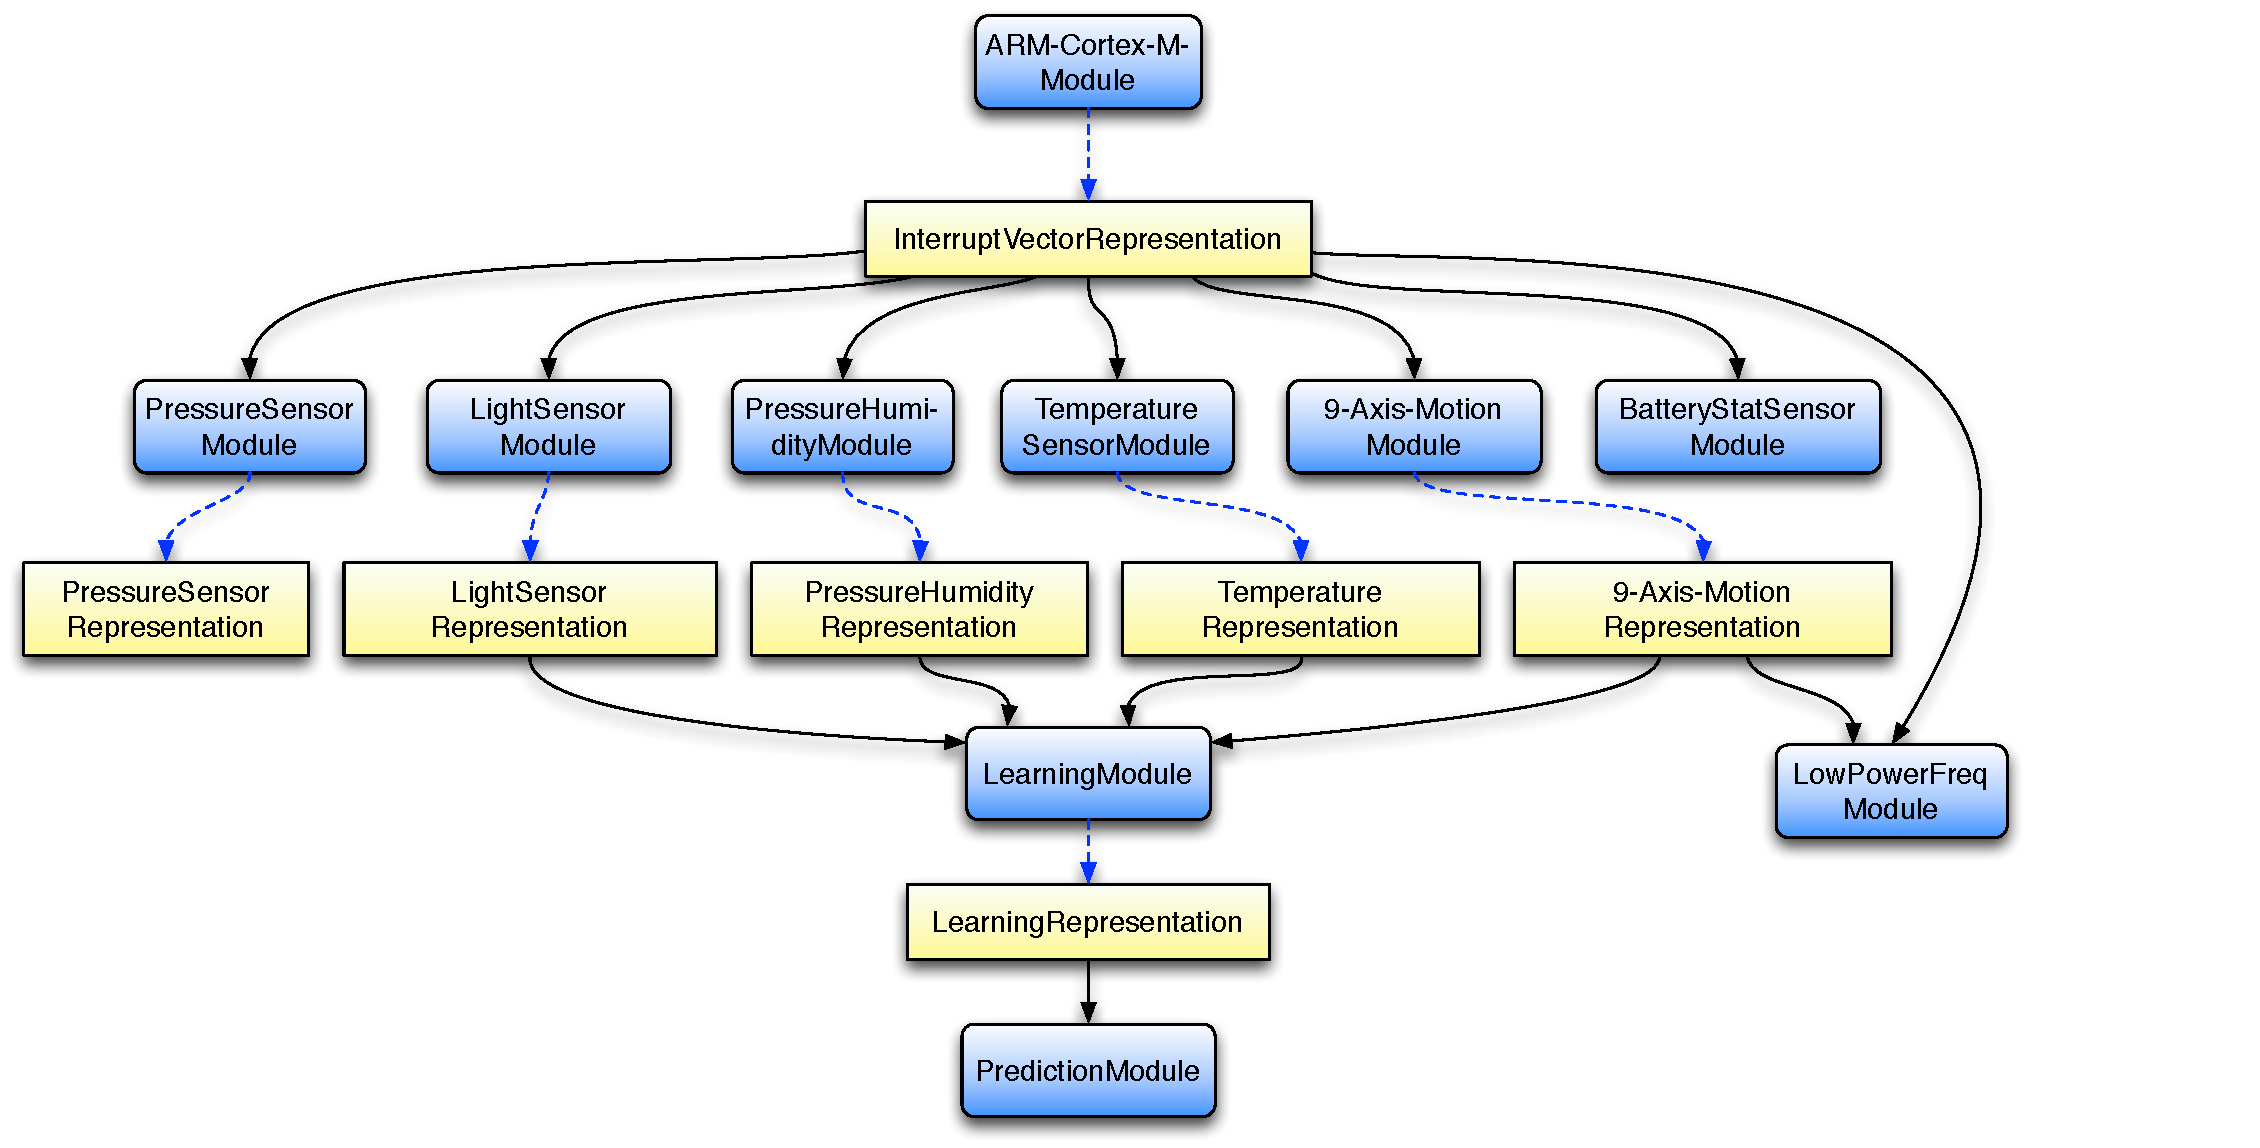
\includegraphics[width=0.5\textwidth]{figures/graph_structure_def-crop3}
\end{figure}
\end{tcolorbox}

%	\begin{block}{Frameworks}
%		\begin{figure*}
%			\centering
%			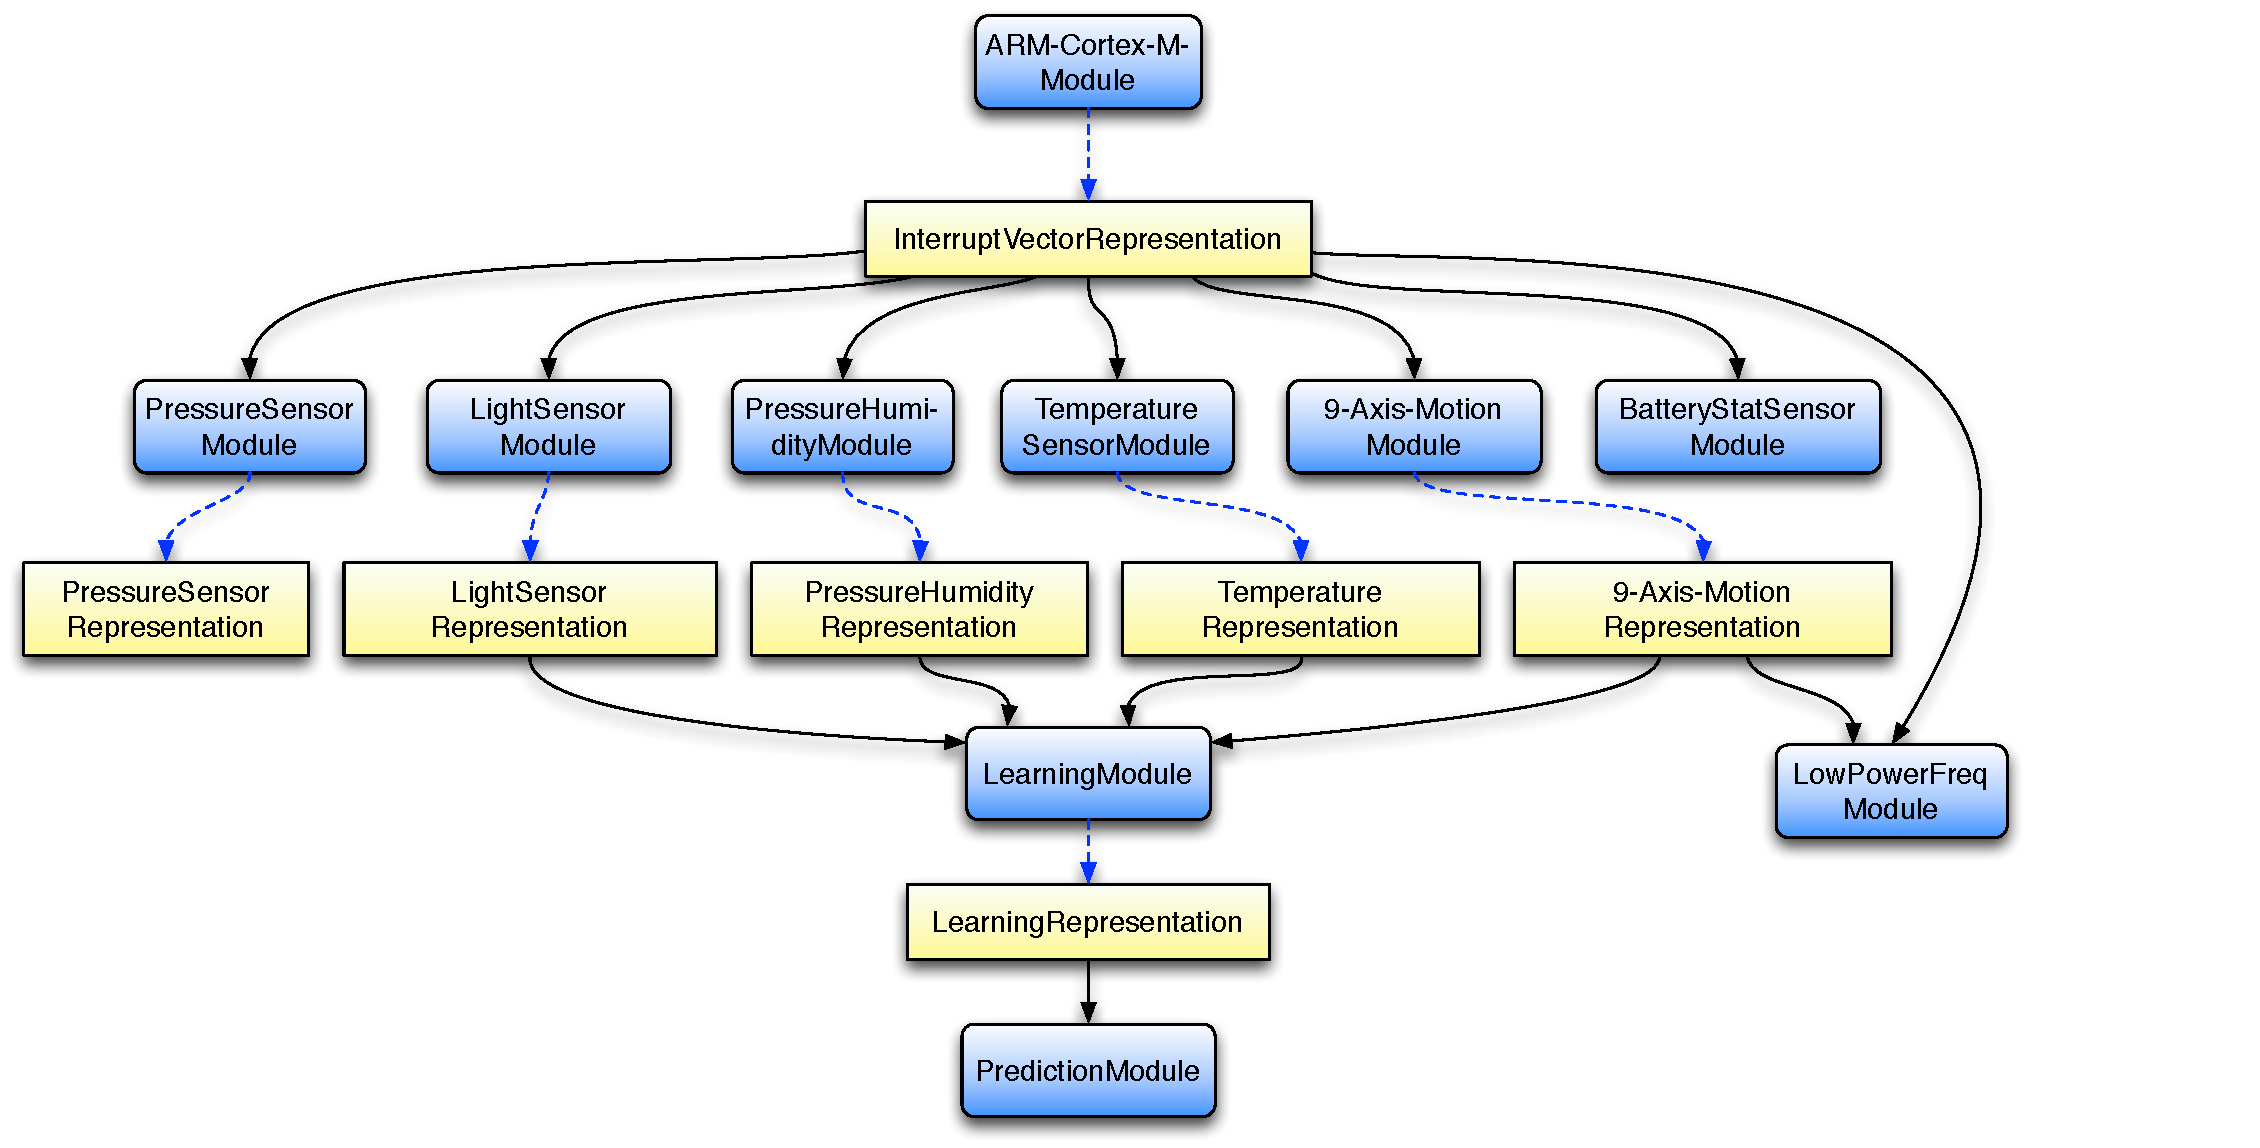
\includegraphics[width=0.6\textwidth]{figures/graph_structure_def-crop3}
%			\includegraphics[width=0.21\textwidth]{figures/human_figure}
%			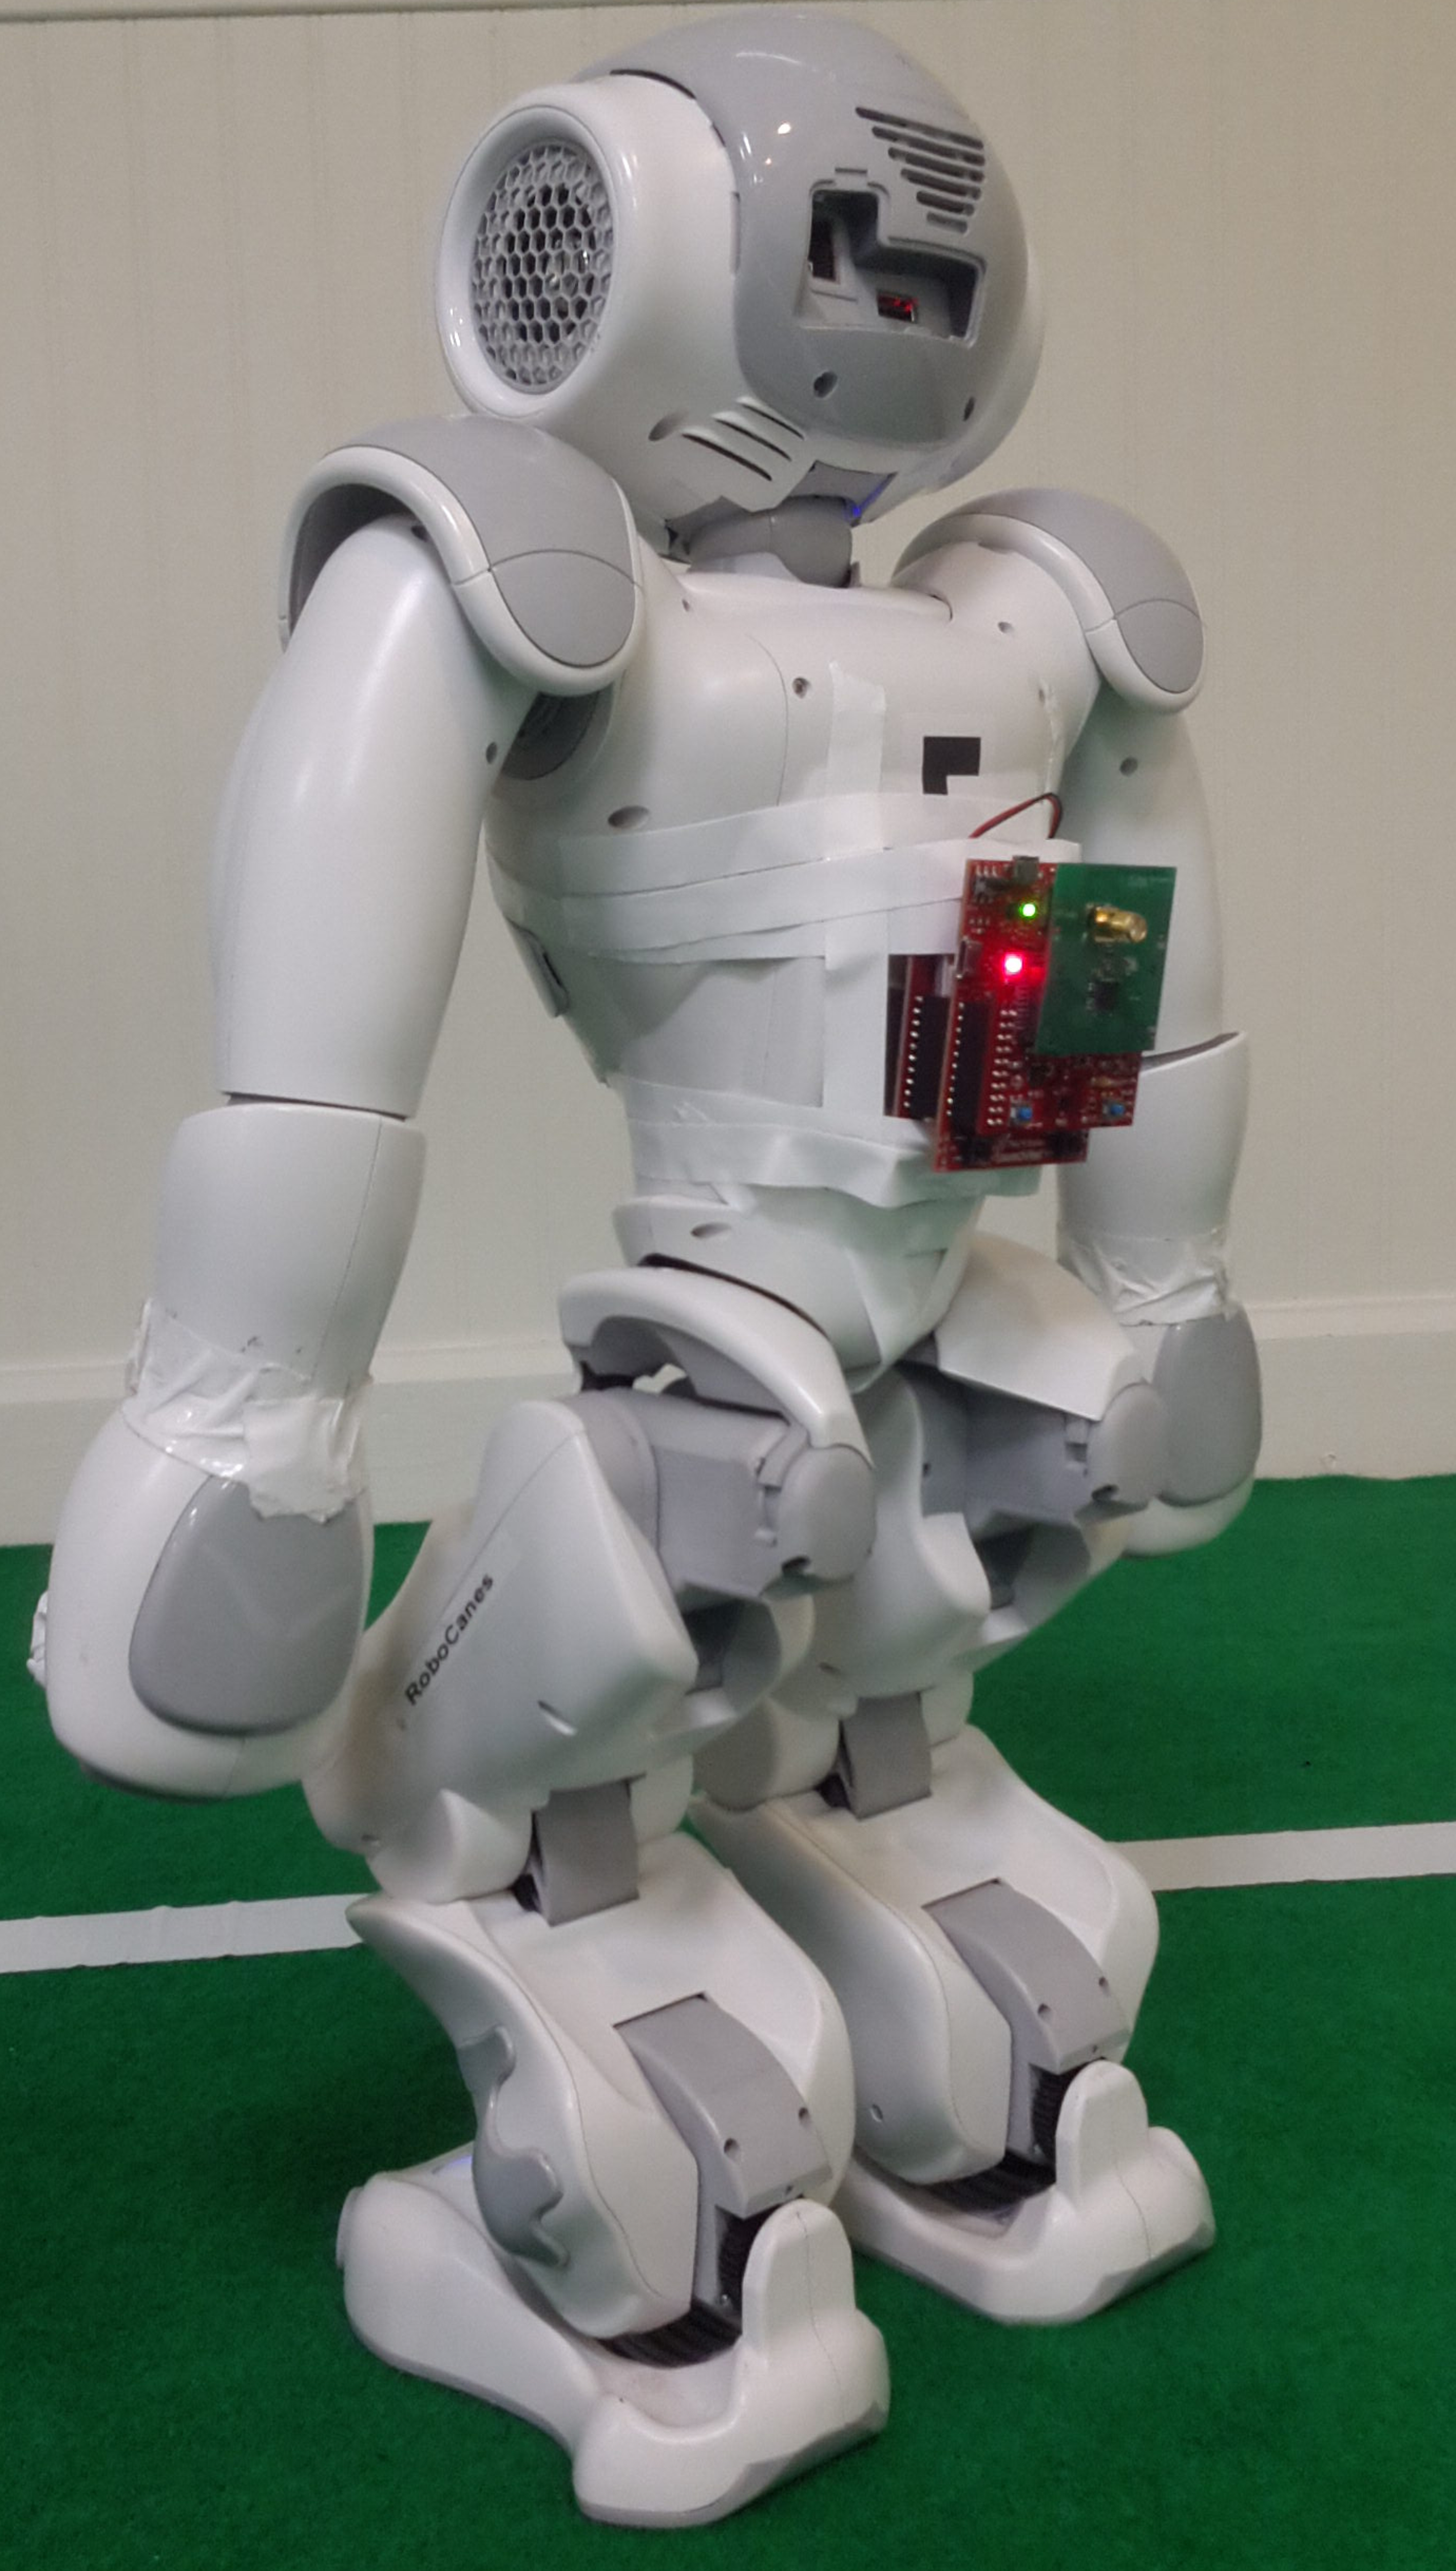
\includegraphics[width=0.185\textwidth]{figures/robot_figure}
%			\label{fig:framework}
%			\caption{(a) Currently available software modules in our framework and a 	
%directed-graph representation of their functional
%				relationship; (b) a wireless sensor device attached to the back of a human subject 
%(c) the same device configuration was used on the back of a NAO
%				humanoid robot.}
%		\end{figure*}
%	\end{block}
}
%%%%%%%%%%%%%%%%%%%%%%%%%%%%%%%%%%%%%%%%%%%%%%%%%%%%%%%%%%%%%



\section{Experimental Setup}
\subsection{Activity Annotation}

\frame{
	\frametitle{Activity Annotation}
	\setbeamercovered{transparent}
	
	\begin{tcolorbox}[colback=white!5,colframe=darkgreen!90!black]
		\begin{figure}
		    \centering
		    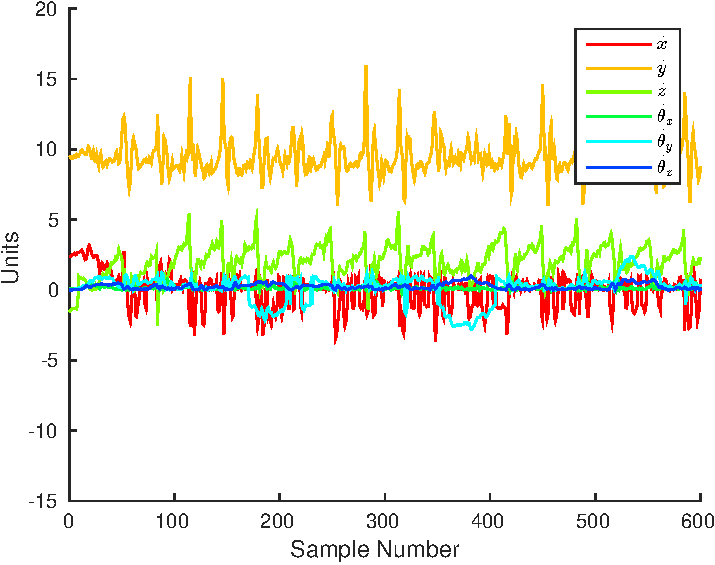
\includegraphics[width=0.4\textwidth]{plots/human_walk2-crop.pdf}
		\end{figure}
		\end{tcolorbox}
	
	
	\begin{tcolorbox}[colback=white!5,colframe=darkgreen!90!black]
	\begin{figure}
	    \centering
	    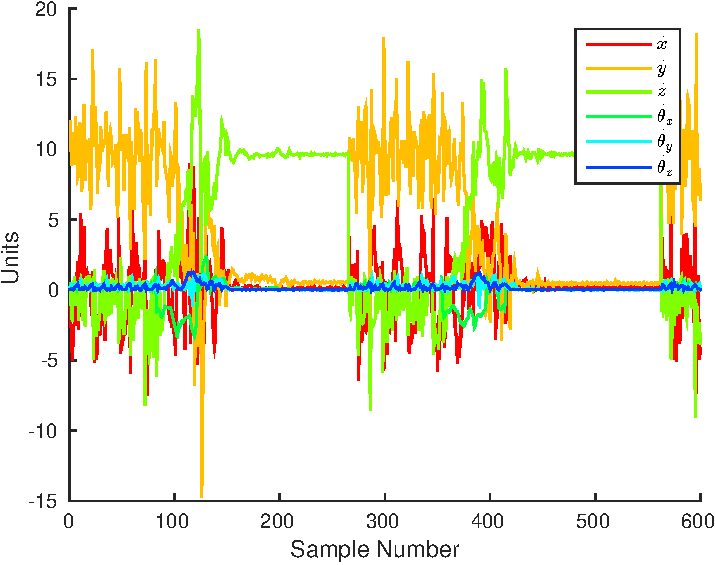
\includegraphics[width=0.4\textwidth]{plots/robot_fallen_forward2-crop.pdf}
	\end{figure}
	\end{tcolorbox}
%	 
%	\begin{block}{Activity Annotation}
%		\begin{figure*}
%			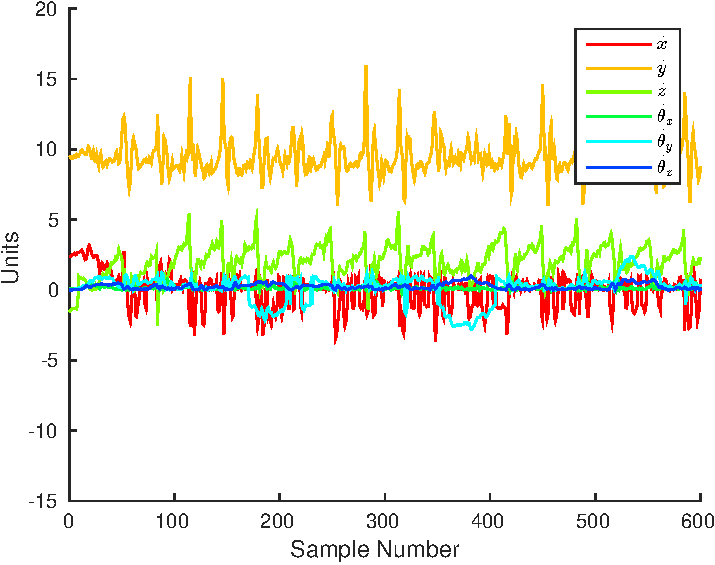
\includegraphics[width=0.25\textwidth]{plots/human_walk2-crop.pdf}
%			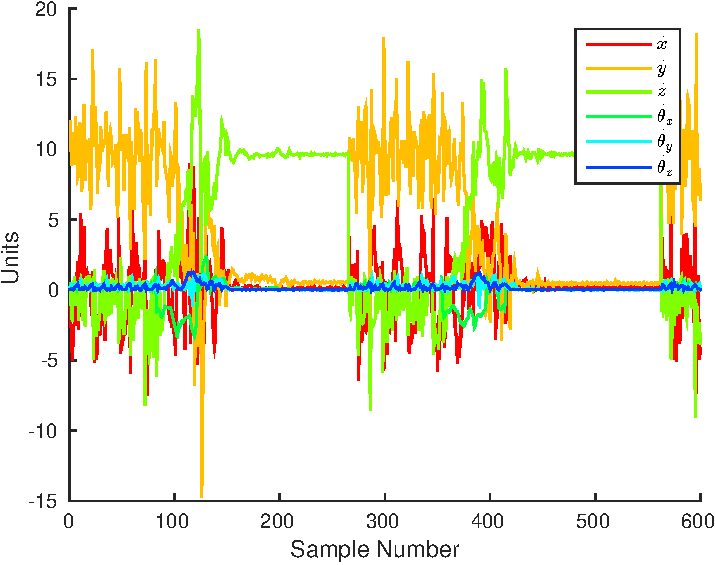
\includegraphics[width=0.25\textwidth]{plots/robot_fallen_forward2-crop.pdf}
%			\caption{Figures (a) shows 3-axis accelerometer and 3-axis gyroscope graph for human 
%motions walking forward Figures (b) shows 3-axis accelerometer and 3-axis gyroscope graph for 
%robot's fallen forward and backward motions.}
%			\label{fig:anotation-human-robot} 
%		\end{figure*}
%		
%	\end{block}
}

%%%%%%%%%%%%%%%%%%%%%%%%%%%%%%%%%%%%%%%%%%%%%%%%%%%%%%%%%%%%%



\section{Evaluation Results}
\subsection{Feature Extraction}
\subsection{Experiments with a Human}
\subsection{Experiments with a NAO Robot}

\frame{
	\frametitle{Evaluation Results}
	\setbeamercovered{transparent} 
	
	\begin{tcolorbox}[colback=green!5,colframe=darkgreen!90!black,title=Feature Extraction]
	\begin{itemize}
			\item 50$Hz$ sampling rate. 
			\item In order to identify activities: 
			\begin{enumerate} 
			\item Window size of $400ms$ (20 	samples); and 
			\item Allowed 10 samples ($200ms$) to overlap between 
					windows. 
				\end{enumerate} 
				\item The selection of the window size is based on the observation that transition 
				from routine  activities to a fall event 
				takes between $180-250ms$. 
				\item Thus, a window size of $400ms$ will include both fall event and 
				non-fall event data for classification
			\end{itemize}
	\end{tcolorbox}
	
	
}

%%%%%%%%%%%%%%%%%%%%%%%%%%%%%%%%%%%%%%%%%%%%%%%%%%%%%%%%%%%%%
\frame{
	\frametitle{Evaluation Results}
	\setbeamercovered{transparent}
	\begin{tcolorbox}[colback=green!5,colframe=darkgreen!90!black,title=Experiments with a Human]
	We have conducted twelve motions in total on the human subject. 
			
			\begin{table}[!ht]
				
				\label{tab:human-logistic-class}
				\centering
				\scalebox{0.65}{
					\begin{tabular} {| l | c | c | c| c|| c| c| c| c|}
						\hline
						& \multicolumn{4}{c||}{\bf Logistic regression} & \multicolumn{4}{c|}{\bf 
						SVM classification} \\ 
						\hline
						{\bf Activity} & {\bf  TP}  &	{\bf TN}  &	{\bf FP} &	{\bf FN}& {\bf  
						TP}  &	{\bf TN}  &	{\bf FP} &	{\bf FN} \\ 
						\hline
						Walking forward	& 91\%	& 90\%	& 10\%	& 9\% & 96\%	& 93\%	& 7\%	& 
						4\% \\ \hline
						Walking backward	& 82\%	& 86\%	& 14\%	& 18\% & 81\%	& 84\%	& 16\%	
						& 19\% \\ \hline
						Walking left 	& 86\%	& 86\%	& 14\%	& 14\% & 89\%	& 90\%	& 10\%	& 
						11\% \\ \hline
						Walking right 	& 86\%	& 86\%	& 14\%	& 14\% & 89\%	& 90\%	& 10\%	& 
						11\% \\ \hline
						Falling forward	& 94\%	& 93\%	& 7\%	& 6\% & 96\%	& 93\%	& 7\%	& 
						4\%	 \\ \hline
						Falling Backward	& 84\%	& 88\%	& 12\%	& 16\%	& 84\%	& 87\%	& 13\%	
						& 16\% \\ \hline
						Falling left	& 92\%	& 91\%	& 9\%	& 8\%	& 93\%	& 93\%	& 7\%	& 
						7\% \\ \hline
						Falling Right	& 92\%	& 91\%	& 9\%	& 8\%	& 92\%	& 93\%	& 7\%	& 
						8\% \\ \hline
						Marching	& 91\%	& 90\%	& 10\%	& 9\%	& 95\%	& 93\%	& 7\%	& 5\% 
						\\ \hline
						Rotate counter-clockwise	& 91\%	& 89\%	& 11\%	& 9\%	& 93\%	& 91\%	
						& 9\%	& 7\%	 \\ \hline
						Rotate clockwise	& 92\%	& 89\%	& 11\%	& 8\%	& 94\%	& 91\%	& 9\%	
						& 6\% \\ \hline
						Stand to seat	& 96\%	& 92\%	& 8\%	& 4\%	& 96\%	& 92\%	& 8\%	& 
						4\%	 \\ \hline
					\end{tabular}
				}
				\caption{Logistic regression and SVM classification for human activities.}
			\end{table}
	
	\end{tcolorbox} 
	
	
}


%%%%%%%%%%%%%%%%%%%%%%%%%%%%%%%%%%%%%%%%%%%%%%%%%%%%%%%%%%%%%
\frame{
	\frametitle{Evaluation Results}
	\setbeamercovered{transparent} 
	\begin{tcolorbox}[colback=green!5,colframe=darkgreen!90!black,title=Kalman Filtering]
	\begin{itemize}
				\item Threshold-based decision making; filtered the roll, pitch, and
				yaw values using a Kalman filter.
				\item If filtered roll values are within $[90\pm15^{\circ}]$ and the filtered pitch 
				values are within  $[0\pm15]^{\circ}$, then with 100\% 
				accuracy, the NAO  robot will be in a normal state. Otherwise the robot 
				is in a fallen state.
				\item If the filtered roll value is less that $60^{\circ}$ 
				, the robot is falling forward. If the filtered roll values is 
				more than 100$^{\circ}$, then it is falling backward.
				\item If the filtered pitch value is less than -50$^{\circ}$, the robot is falling 
				to the left side, while if the 
				filtered pitch values is more than 50$^{\circ}$,then it is falling to the right 
				side.
				\item  With these thresholds for a separate test cases, the thresholding method has 
				detected fallen 				state with 100\% accuracy. 
			\end{itemize}
	\end{tcolorbox}
	
	
}

%%%%%%%%%%%%%%%%%%%%%%%%%%%%%%%%%%%%%%%%%%%%%%%%%%%%%%%%%%%%%
\subsubsection*{Experiments with a NAO Robot}
%\frame{
%	\frametitle{Evaluation Results}
%	\setbeamercovered{transparent} 
%	\begin{block}{Kalman Filtering}
%		\begin{figure*}
%			\includegraphics[width=0.25\textwidth]
%				{figures/plot1-crop}
%			\includegraphics[width=0.25\textwidth]
%				{figures/plot5-crop}
%			\includegraphics[width=0.25\textwidth]
%				{figures/plot1_fallen-crop}
%			\includegraphics[width=0.25\textwidth]
%				{figures/plot2_fallen-crop}
%			\caption{Figures (a--b) show the roll and pitch angles (raw and filtered) for normal 
%				behaviors marching in place and walking backward. Figures (c--d) show the raw and 
%filtered roll 
%				and pitch angles for fallen forward and backwards states of NAO humanoid robot.}
%			\label{fig:normalFallenBehavior}
%		\end{figure*}
%	\end{block}
%}

%%%%%%%%%%%%%%%%%%%%%%%%%%%%%%%%%%%%%%%%%%%%%%%%%%%%%%%%%%%%%
\frame{
	\frametitle{Evaluation Results}
	\setbeamercovered{transparent}
	
	\begin{tcolorbox}[colback=green!5,colframe=darkgreen!90!black,title=Experiments with a NAO 
	Robot]
	We have conducted eleven motions in total on the robot subject. 
			\begin{table}[!ht]
				
				\label{tab:robot-logistic-class}
				\centering
				\scalebox{0.65}{
					\begin{tabular} {| l | c | c | c| c|| c| c| c| c|}
						\hline
						& \multicolumn{4}{c||}{\bf Logistic regression} & \multicolumn{4}{c|}{\bf 
						SVM classification} \\ 
						\hline
						{\bf Activity} & {\bf  TP}  &	{\bf TN}  &	{\bf FP} &	{\bf FN}& {\bf  
						TP}  &	{\bf TN}  &	{\bf FP} &	{\bf FN} \\ 
						\hline
						Walking forward	& 91\%	& 90\%	& 10\%	& 9\% & 93\%	& 91\%	& 9\%	& 7 
						\% \\ \hline
						Walking backward	& 90\%	& 90\%	& 10\%	& 10\% & 93\%	& 91\%	& 9\%	
						& 7\% \\ \hline
						Walking left 	& 92\%	& 90\%	& 10\%	& 8\%  & 94\%	& 90\%	& 10\%	& 
						6\% \\ \hline
						Walking right 	& 89\%	& 90\%	& 10\%	& 11\% & 90\%	& 91\%	& 9\%	& 
						10\% \\ \hline
						Falling forward	& 94\%	& 93\%	& 7\%	& 6\%	& 98\%	& 93\%	& 7\%	& 
						2\% \\ \hline
						Falling Backward	& 94\%	& 93\%	& 7\%	& 6\%	 & 98\%	& 93\%	& 7\%	
						& 2\% \\ \hline
						Falling left	& 95\%	& 93\%	& 7\%	& 5\%	& 99\%	& 94\%	& 6\%	& 
						1\% \\ \hline
						Falling Right	& 94\%	& 93\%	& 7\%	& 6\%	& 98\%	& 93\%	& 7\%	& 
						2\%	 \\ \hline
						Marching	& 91\%	& 89\%	& 11\%	& 9\%	& 90\%	& 91\%	& 11\%	& 
						10\%	 \\ \hline
						Rotate counter-clockwise	& 97\%	& 92\%	& 8\%	& 3\%	& 97\%	& 93\%	
						& 7\%	& 3\%	 \\ \hline
						Rotate clockwise	& 98\%	& 92\%	& 8\%	& 2\%	& 96\%	& 93\%	& 7\%	
						& 4\%	 \\ \hline
					\end{tabular}
				}
				\caption{Logistic regression  and SVM classification for robot activities.}
			\end{table}
	\end{tcolorbox}
	
}

%%%%%%%%%%%%%%%%%%%%%%%%%%%%%%%%%%%%%%%%%%%%%%%%%%%%%%%%%%%%%

\section{Conclusion \& Future Work}

\frame{
	\frametitle{Conclusion \& Future Work}
	\setbeamercovered{transparent} 
	\begin{tcolorbox}[colback=green!5,colframe=darkgreen!90!black,title=Conclusion \& Future Work]
	\begin{itemize}
			 \item	Learn and predict different activities for humans and robots
			\item  A generic ramework software tools for	embedded devices.
			\item We were able to detect of falls and other activities with high accuracy.
			\item our future work will be to use multiple sensing devices to create a sensor network.
			\item Detect complex activities with higher sampling rates.
			\end{itemize}
	\end{tcolorbox}
	
}


%%%%%%%%%%%%%%%%%%%%%%%%%%%%%%%%%%%%%%%%%%%%%%%%%%%%%%%%%%%%%

%\section{*Conclusion \& Future Work}
%\subsubsection*{*Conclusion \& Future Work}

\frame{
	\frametitle{}
	\setbeamercovered{transparent}
	\begin{tcolorbox}[colback=green!5,colframe=darkgreen!90!black]
	  \center \huge Thank You
	  \end{tcolorbox} 
}

%%%%%%%%%%%%%%%%%%%%%%%%%%%%%%%%%%%%%%%%%%%%%%%%%%%%%%%%%%%%%

%\section{*Conclusion \& Future Work}
%\subsubsection*{*Conclusion \& Future Work}

%\frame{
%	\frametitle{}
%	\setbeamercovered{transparent} 
%	\begin{block}{}
%		\centering
%		\huge Questions ?
%	\end{block}
%}

\end{document}